% \IUref{IUAdmPS}{Administrar Planta de Selección}
% \IUref{IUModPS}{Modificar Planta de Selección}
% \IUref{IUEliPS}{Eliminar Planta de Selección}


% Copie este bloque por cada caso de uso:
%-------------------------------------- COMIENZA descripción del caso de uso.

%\begin{UseCase}[archivo de imágen]{UCX}{Nombre del Caso de uso}{
	\begin{UseCase}{CU28.0}{Registrar ingreso a área}{
		En esta sección el usuario podrá ingresar al área dependiendo el tipo de membresia que este 				tenga.
	}
		\UCitem{Versión}{1.0}
		\UCitem{Actor}{Usuario}
		\UCitem{Propósito}{Permitir o restringir el acceso de las áreas a los usuarios, tomando como 				base el tipo de membresia que estos tengan.}
		\UCitem{Entradas}{Clave.}
		\UCitem{Origen}{El dato será ingresadas desde un teclado.}
		\UCitem{Salidas}{Mensaje de acceso correcto, Mensaje acceso no permitido, mensaje de 				usuario no identificado.}
		\UCitem{Destino}{El registro será enviado a una base de datos, con un identificador de activo.}
		\UCitem{Precondiciones}{Que el usuario tenga al menos una membresia para poder ingresar a 			alguna área.}
		\UCitem{Postcondiciones}{El actor podrá regresar al menú de opciones para realizar otras operaciones en el sistema.}
		\UCitem{Errores}{Que el sistema no reconozca al usuario identificado.}
		\UCitem{Tipo}{Caso de uso primario}
		\UCitem{Observaciones}{Este tipo de verificación en el sistema de registro ubicado en la 		entrada del gimnasio, posteriormente en cada área se hará una verificación con la clave del usuario para poder tener el acceso a las áreas.}
		\UCitem{Autor}{Francisco García Enríquez.}
		\UCitem{Revisor}{Isaac Fernandez.}
	\end{UseCase}

	\begin{UCtrayectoria}{Principal}
		\UCpaso[\UCactor] El usuario solicita el acceso en el boton ingresar, por medio de una pantalla.
		\UCpaso El sistema muestra un login de acceso, los datos que se muestran son: Nombre de 				usuario y Clave.
		\UCpaso[\UCactor] Ingresa su usuario.
		\UCpaso[\UCactor] Confirma su registro.
		\UCpaso Muestra un mensaje de error, {\bf MSG18-}``falta ingresar la Clave.''
		\UCpaso[\UCactor] Ingresa su Clave en campo correspondiente.
		\UCpaso[\UCactor] Confirma su registro.
		\UCpaso Muestra un mensaje {\bf MSG19-}``Acceso Correcto.''
	\end{UCtrayectoria}
%-------------------------------------- TERMINA descripción del caso de uso.

		\begin{UCtrayectoriaA}{A}{El actor no se encuentra registrado en el sistema.}
			\UCpaso[\UCactor] Ingresa su nombre.
			\UCpaso[\UCactor] Ingresa su clave.
			\UCpaso[\UCactor] Confirma el acceso.
			\UCpaso Manda un mensaje  {\bf MSG20-}``Usted no está identificado en el sistema.''
			\UCpaso[\UCactor] Presiona sobre el mensaje error el boton de aceptar.
		\end{UCtrayectoriaA}

\begin{figure}[htbp!]
		\centering
			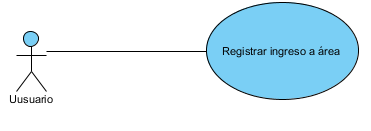
\includegraphics[width=0.8\textwidth]{images/registraIngresoArea}
		\caption{Diagrama de Casos de Uso del sistema.}
	\end{figure}
	